\documentclass{beamer}
\usetheme{metropolis}
\usepackage{graphicx}
\usepackage{subcaption}
\usepackage{hyperref}
\usepackage{tcolorbox}
\title{Algebra-Based Physics-1: Mechanics (PHYS135A): Summary}
\date{\today}
\author{Jordan Hanson}
\institute{Whittier College Department of Physics and Astronomy}

\begin{document}
\maketitle

\section{Review}

\begin{frame}{Summary}
\begin{enumerate}
\item Unit 0 - Units, estimation, and vectors
\item Unit 1 - Kinematics
\item Unit 2 - Kinematics in More than One Dimension
\item Unit 3 - Midterm 1
\item Unit 4 - Newton's Laws of Motion
\item Unit 5 - Applications of Newton's Laws: friction, drag, elasticity
\item Final Project Proposals
\item Unit 6 - Uniform Circular Motion
\item Unit 7 - Work, Energy, and Energy Consumption
\item Unit 8 - Linear Momentum
\item Unit 9 - Rotational Dynamics
\end{enumerate}
\end{frame}

\section{It has been my pleasure.}

\begin{frame}{Oops}
\begin{figure}

\includegraphics[width=0.85\textwidth]{savage.pdf}
\end{figure}
\end{frame}

\begin{frame}{Doctor's Visits}
\begin{figure}
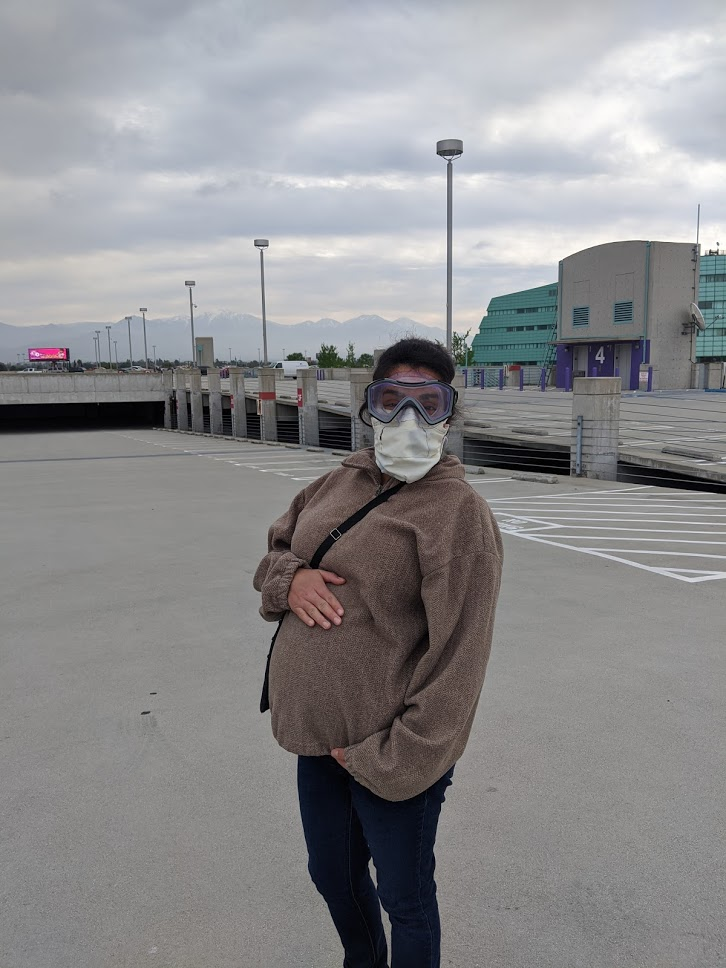
\includegraphics[width=0.5\textwidth]{priscilla1.jpg}
\end{figure}
\end{frame}

\begin{frame}{New Life}
\begin{figure}
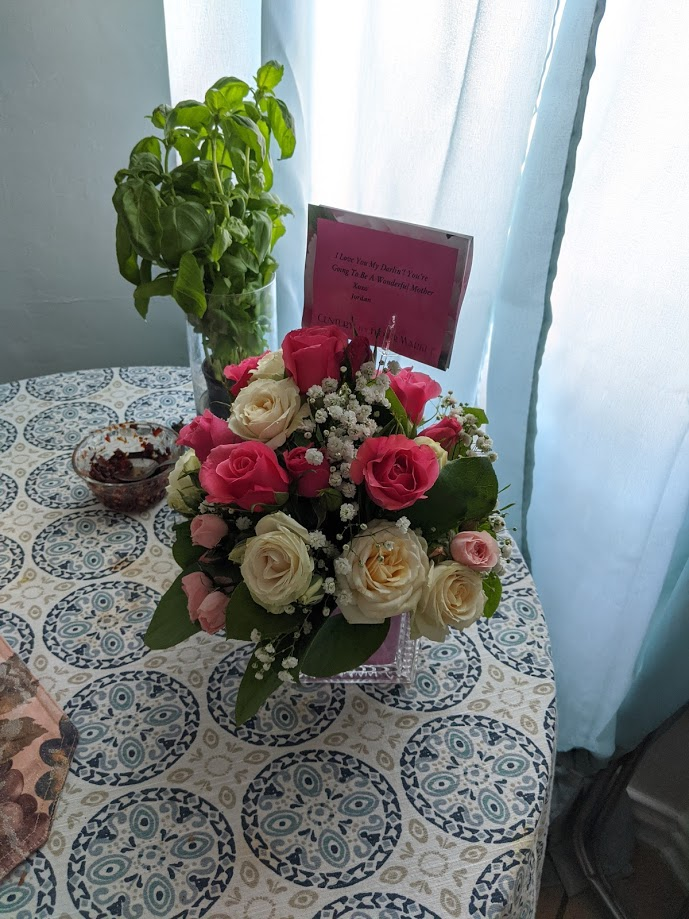
\includegraphics[width=0.5\textwidth]{flowers.jpg}
\end{figure}
\end{frame}

\begin{frame}{East Los Angeles}
\begin{figure}
\includegraphics[width=0.5\textwidth]{birth.jpg}
\end{figure}
\end{frame}

\begin{frame}{Family}
\begin{figure}
\includegraphics[width=0.4\textwidth]{wife.jpg}
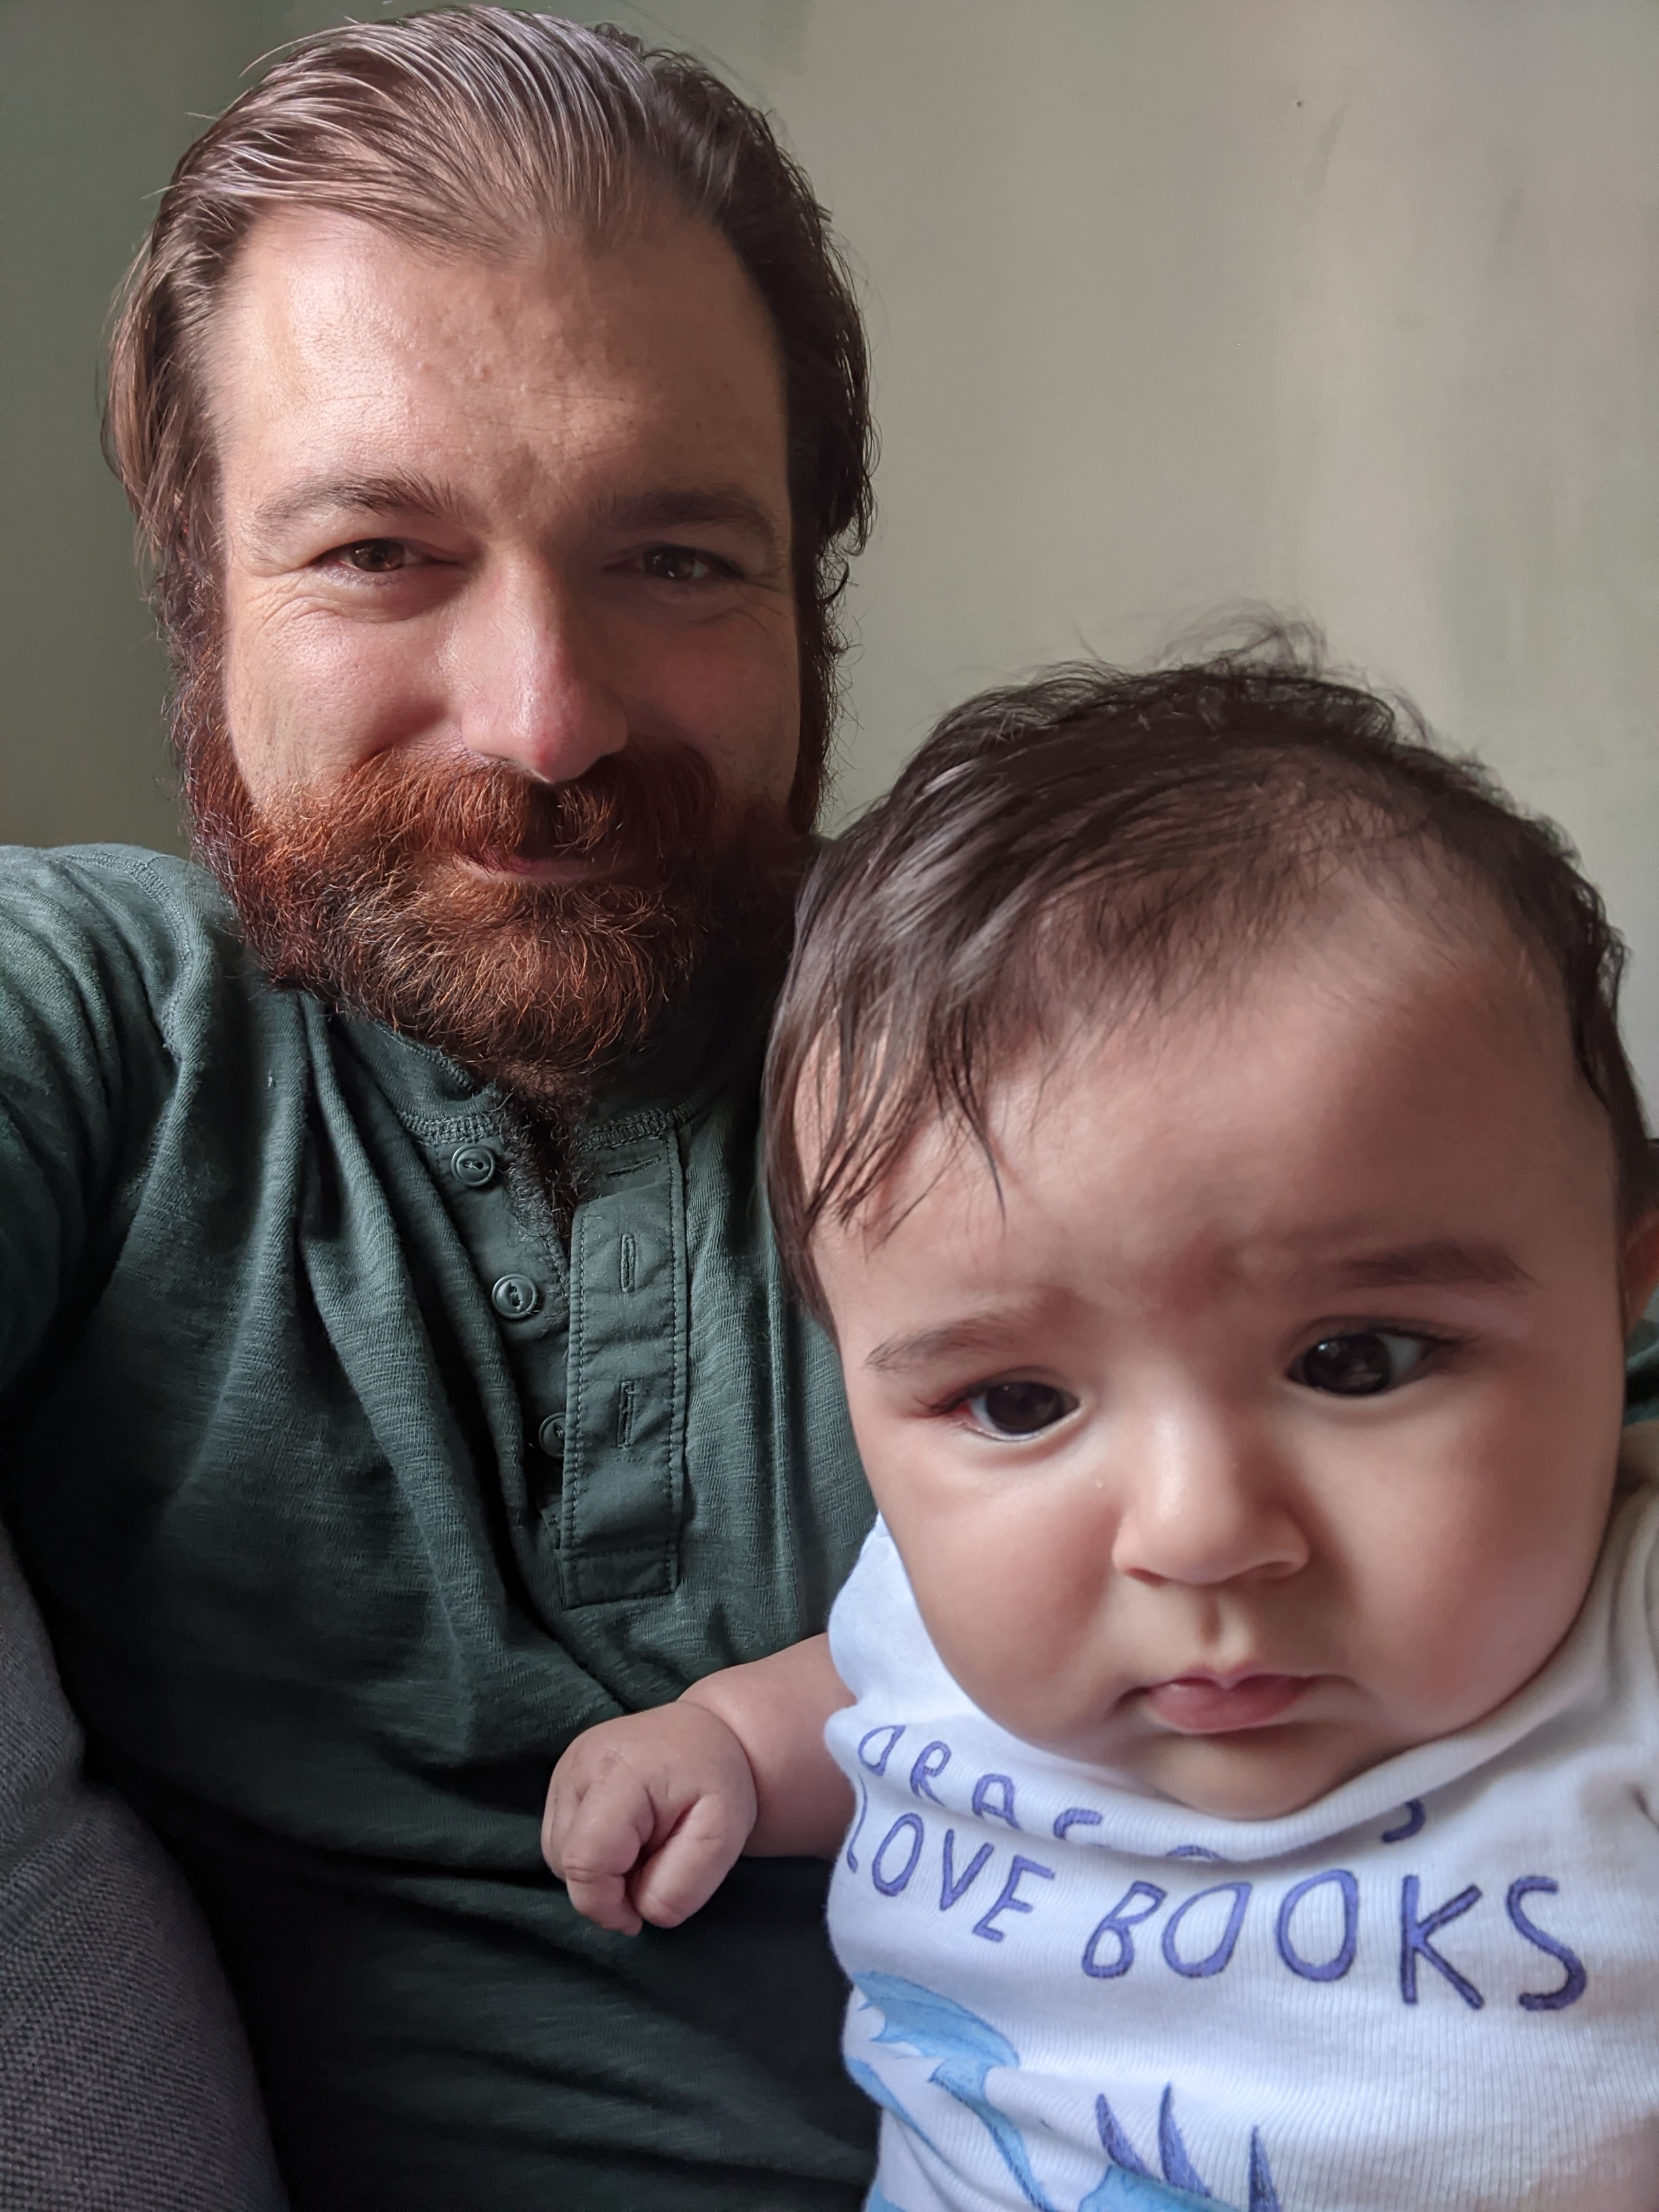
\includegraphics[width=0.4\textwidth]{green.jpg}
\end{figure}
\end{frame}

\begin{frame}{Birthday}
\begin{figure}
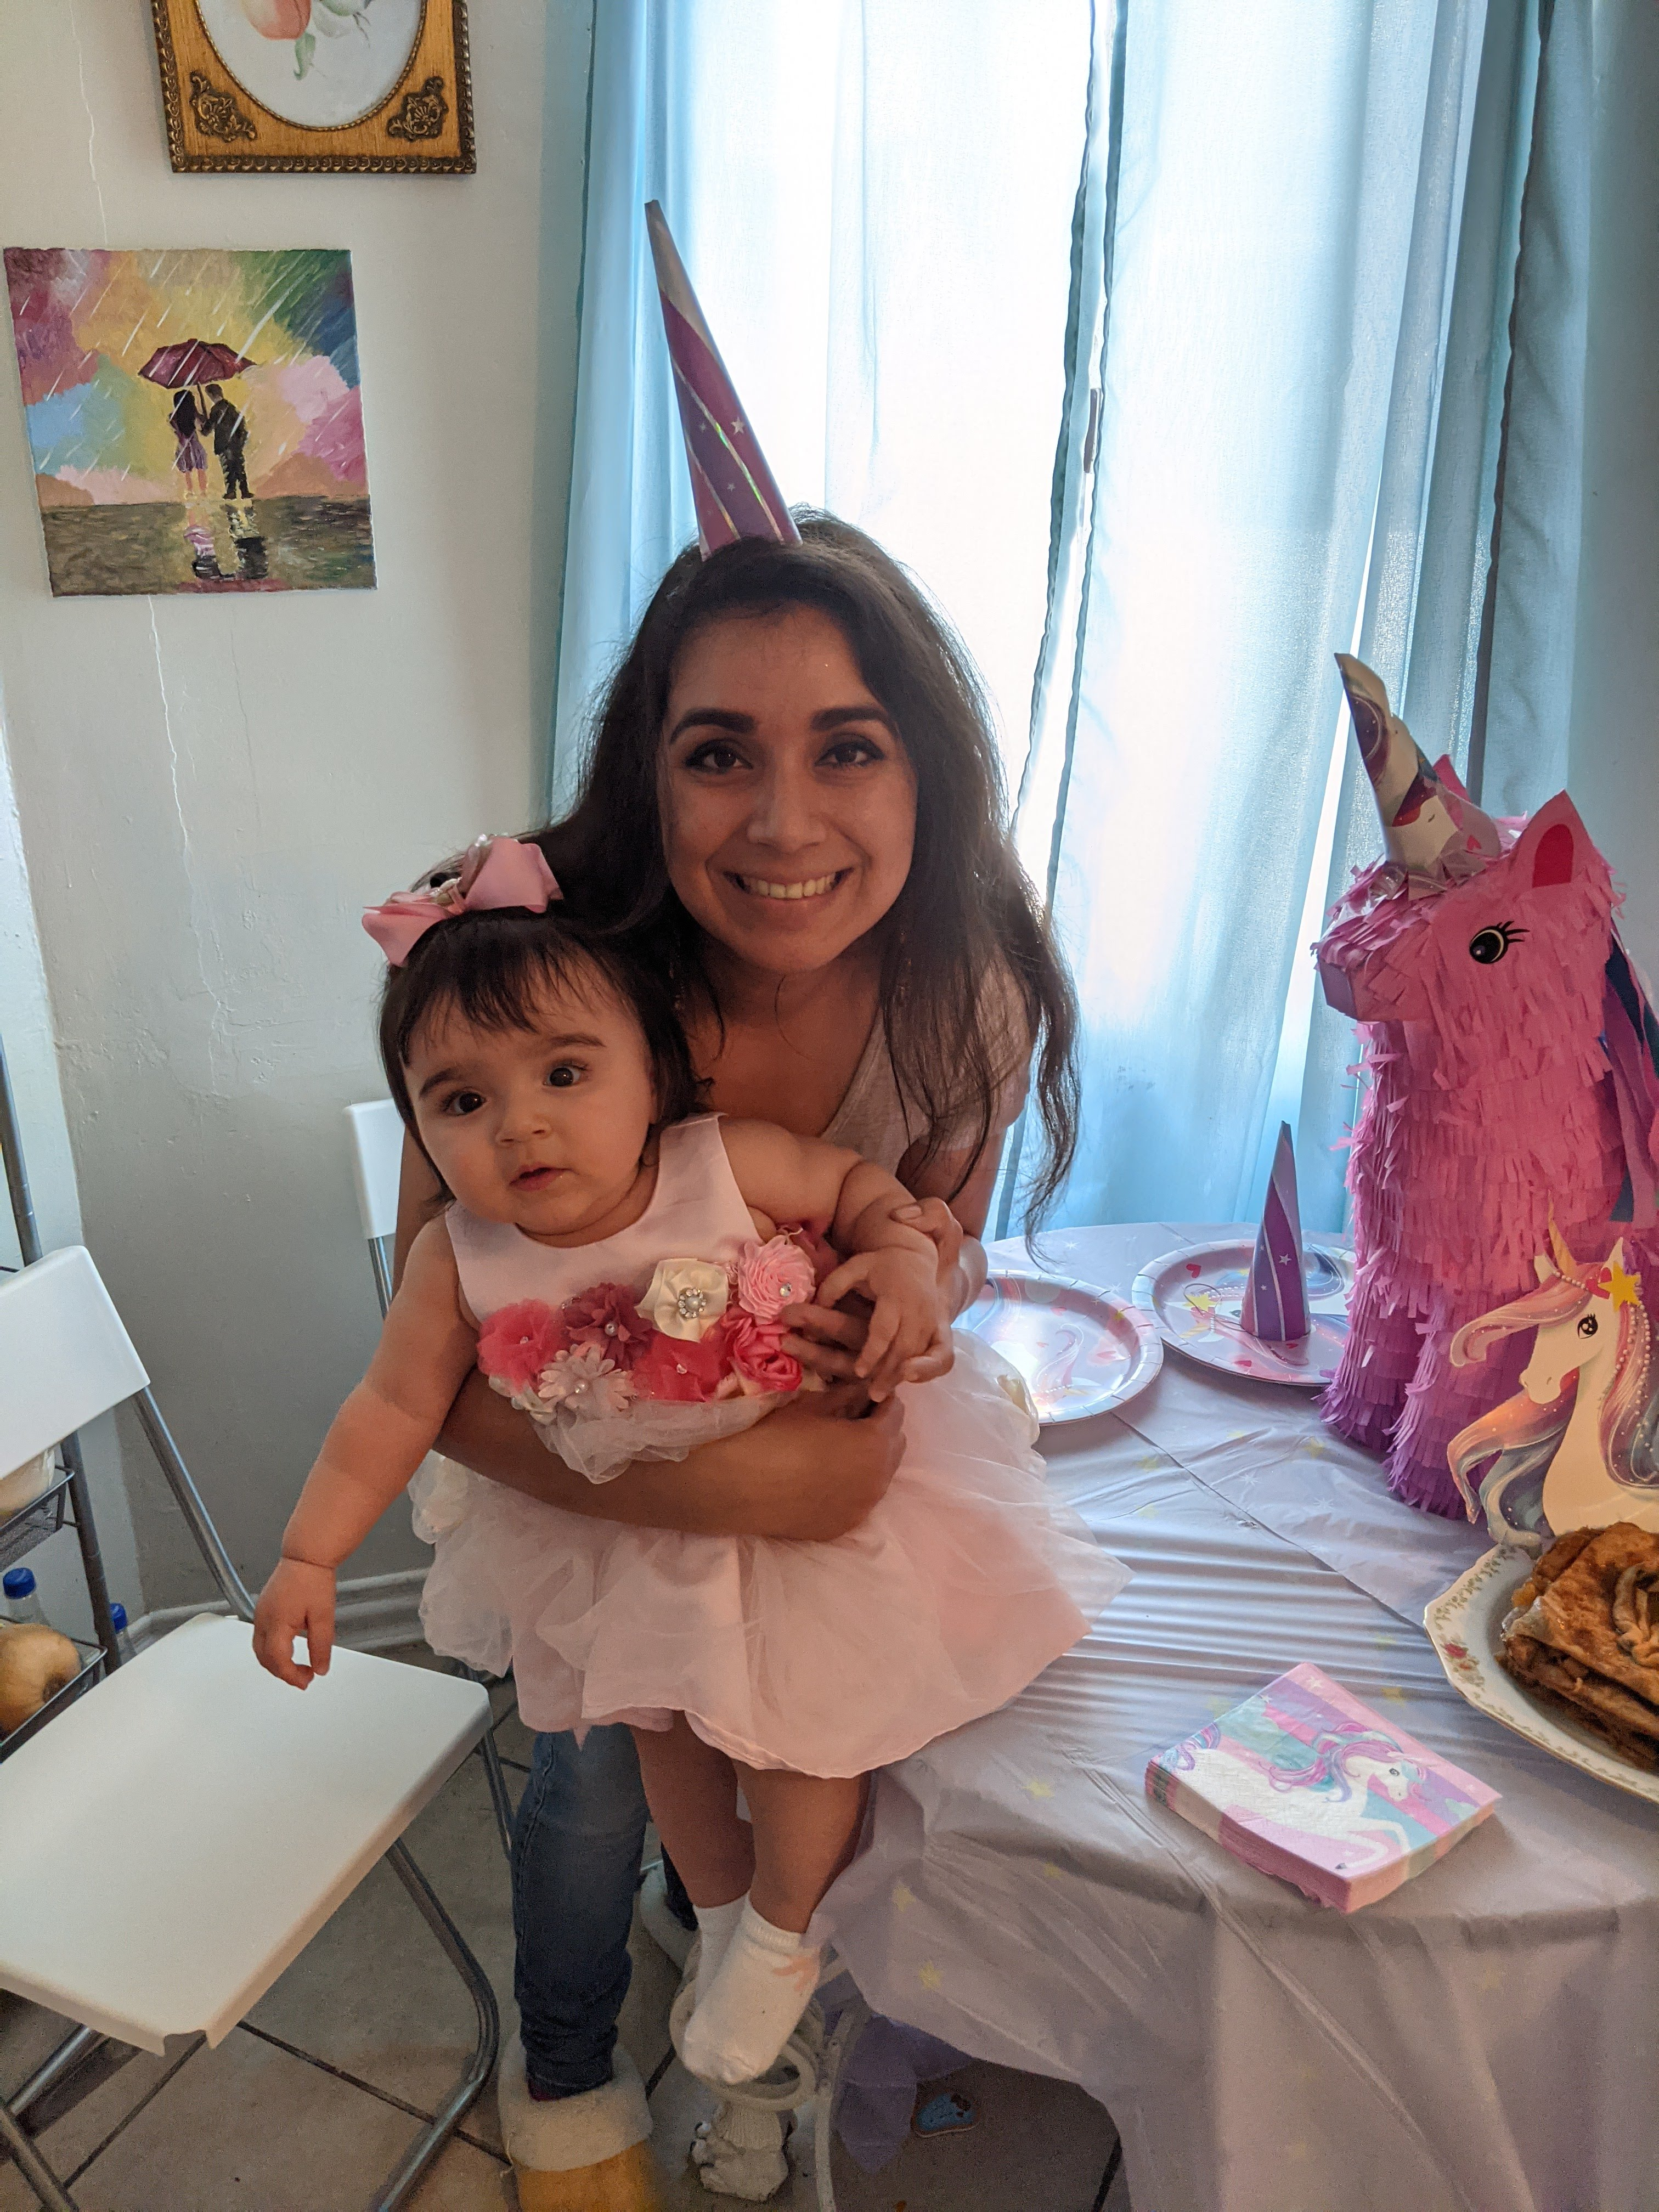
\includegraphics[width=0.5\textwidth]{bday.jpg}
\end{figure}
\end{frame}

\begin{frame}{Work}
\begin{figure}
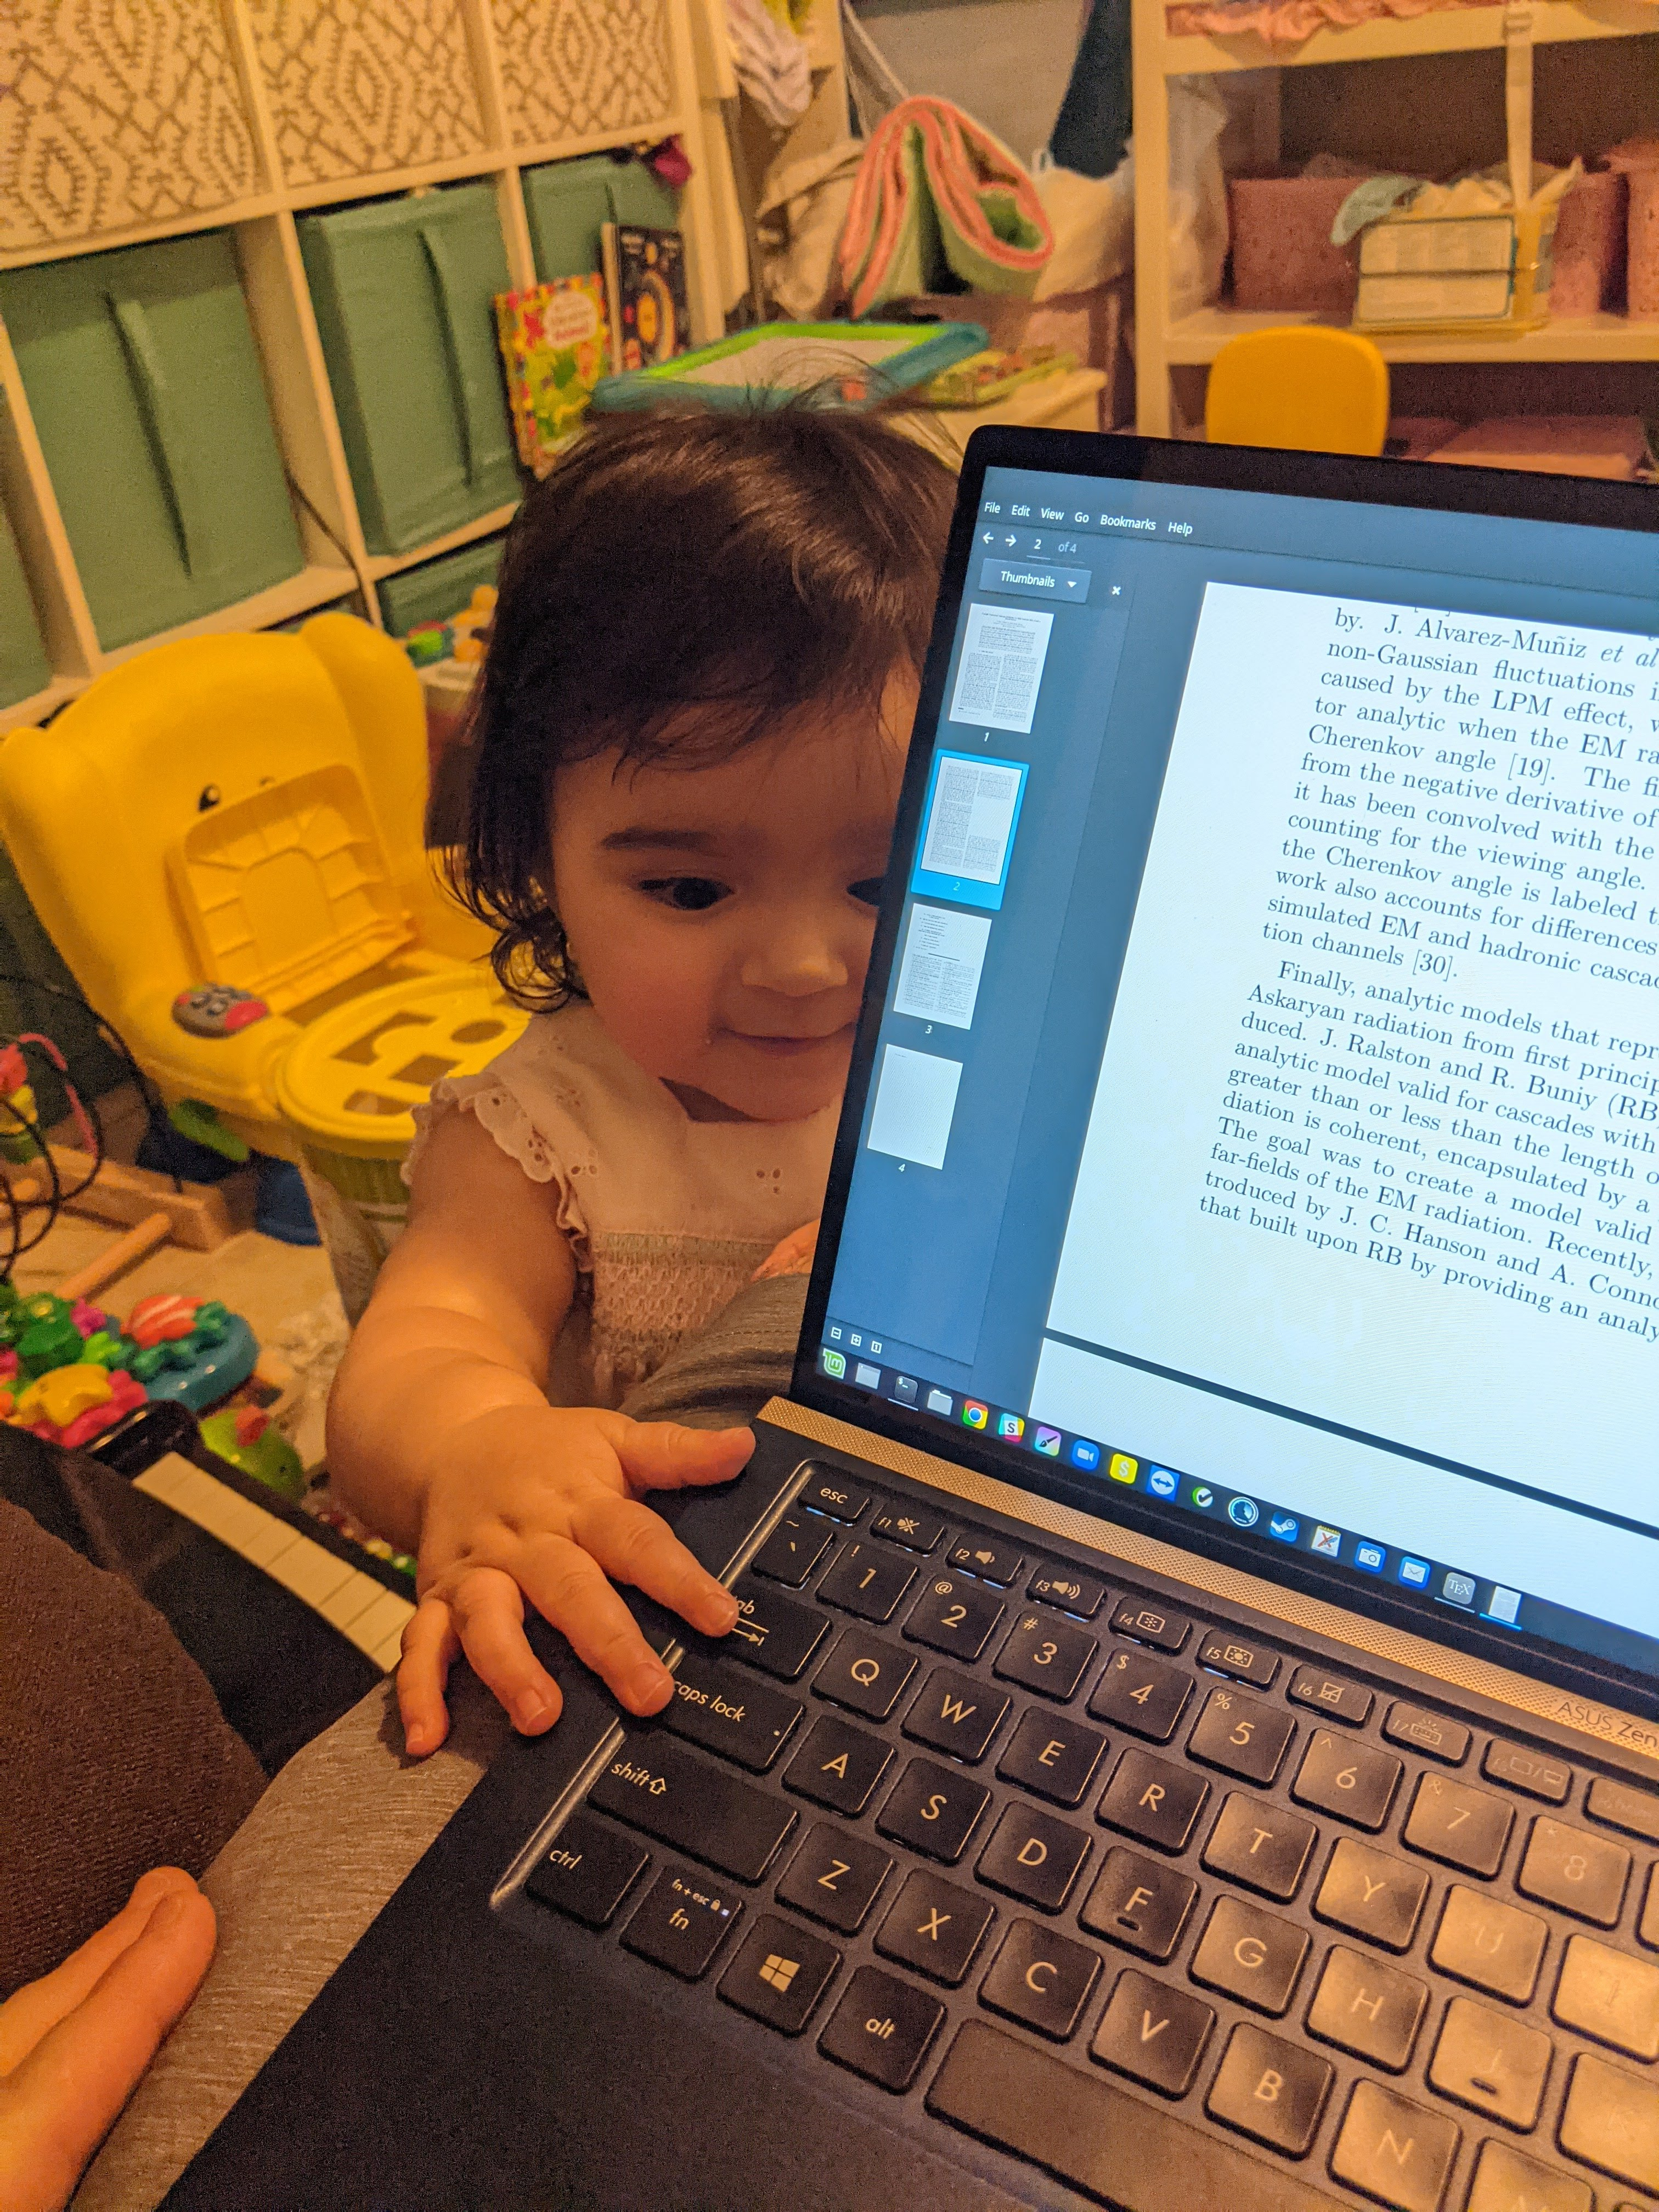
\includegraphics[width=0.5\textwidth]{work.jpg}
\end{figure}
\end{frame}

\begin{frame}{Sleep}
\begin{figure}
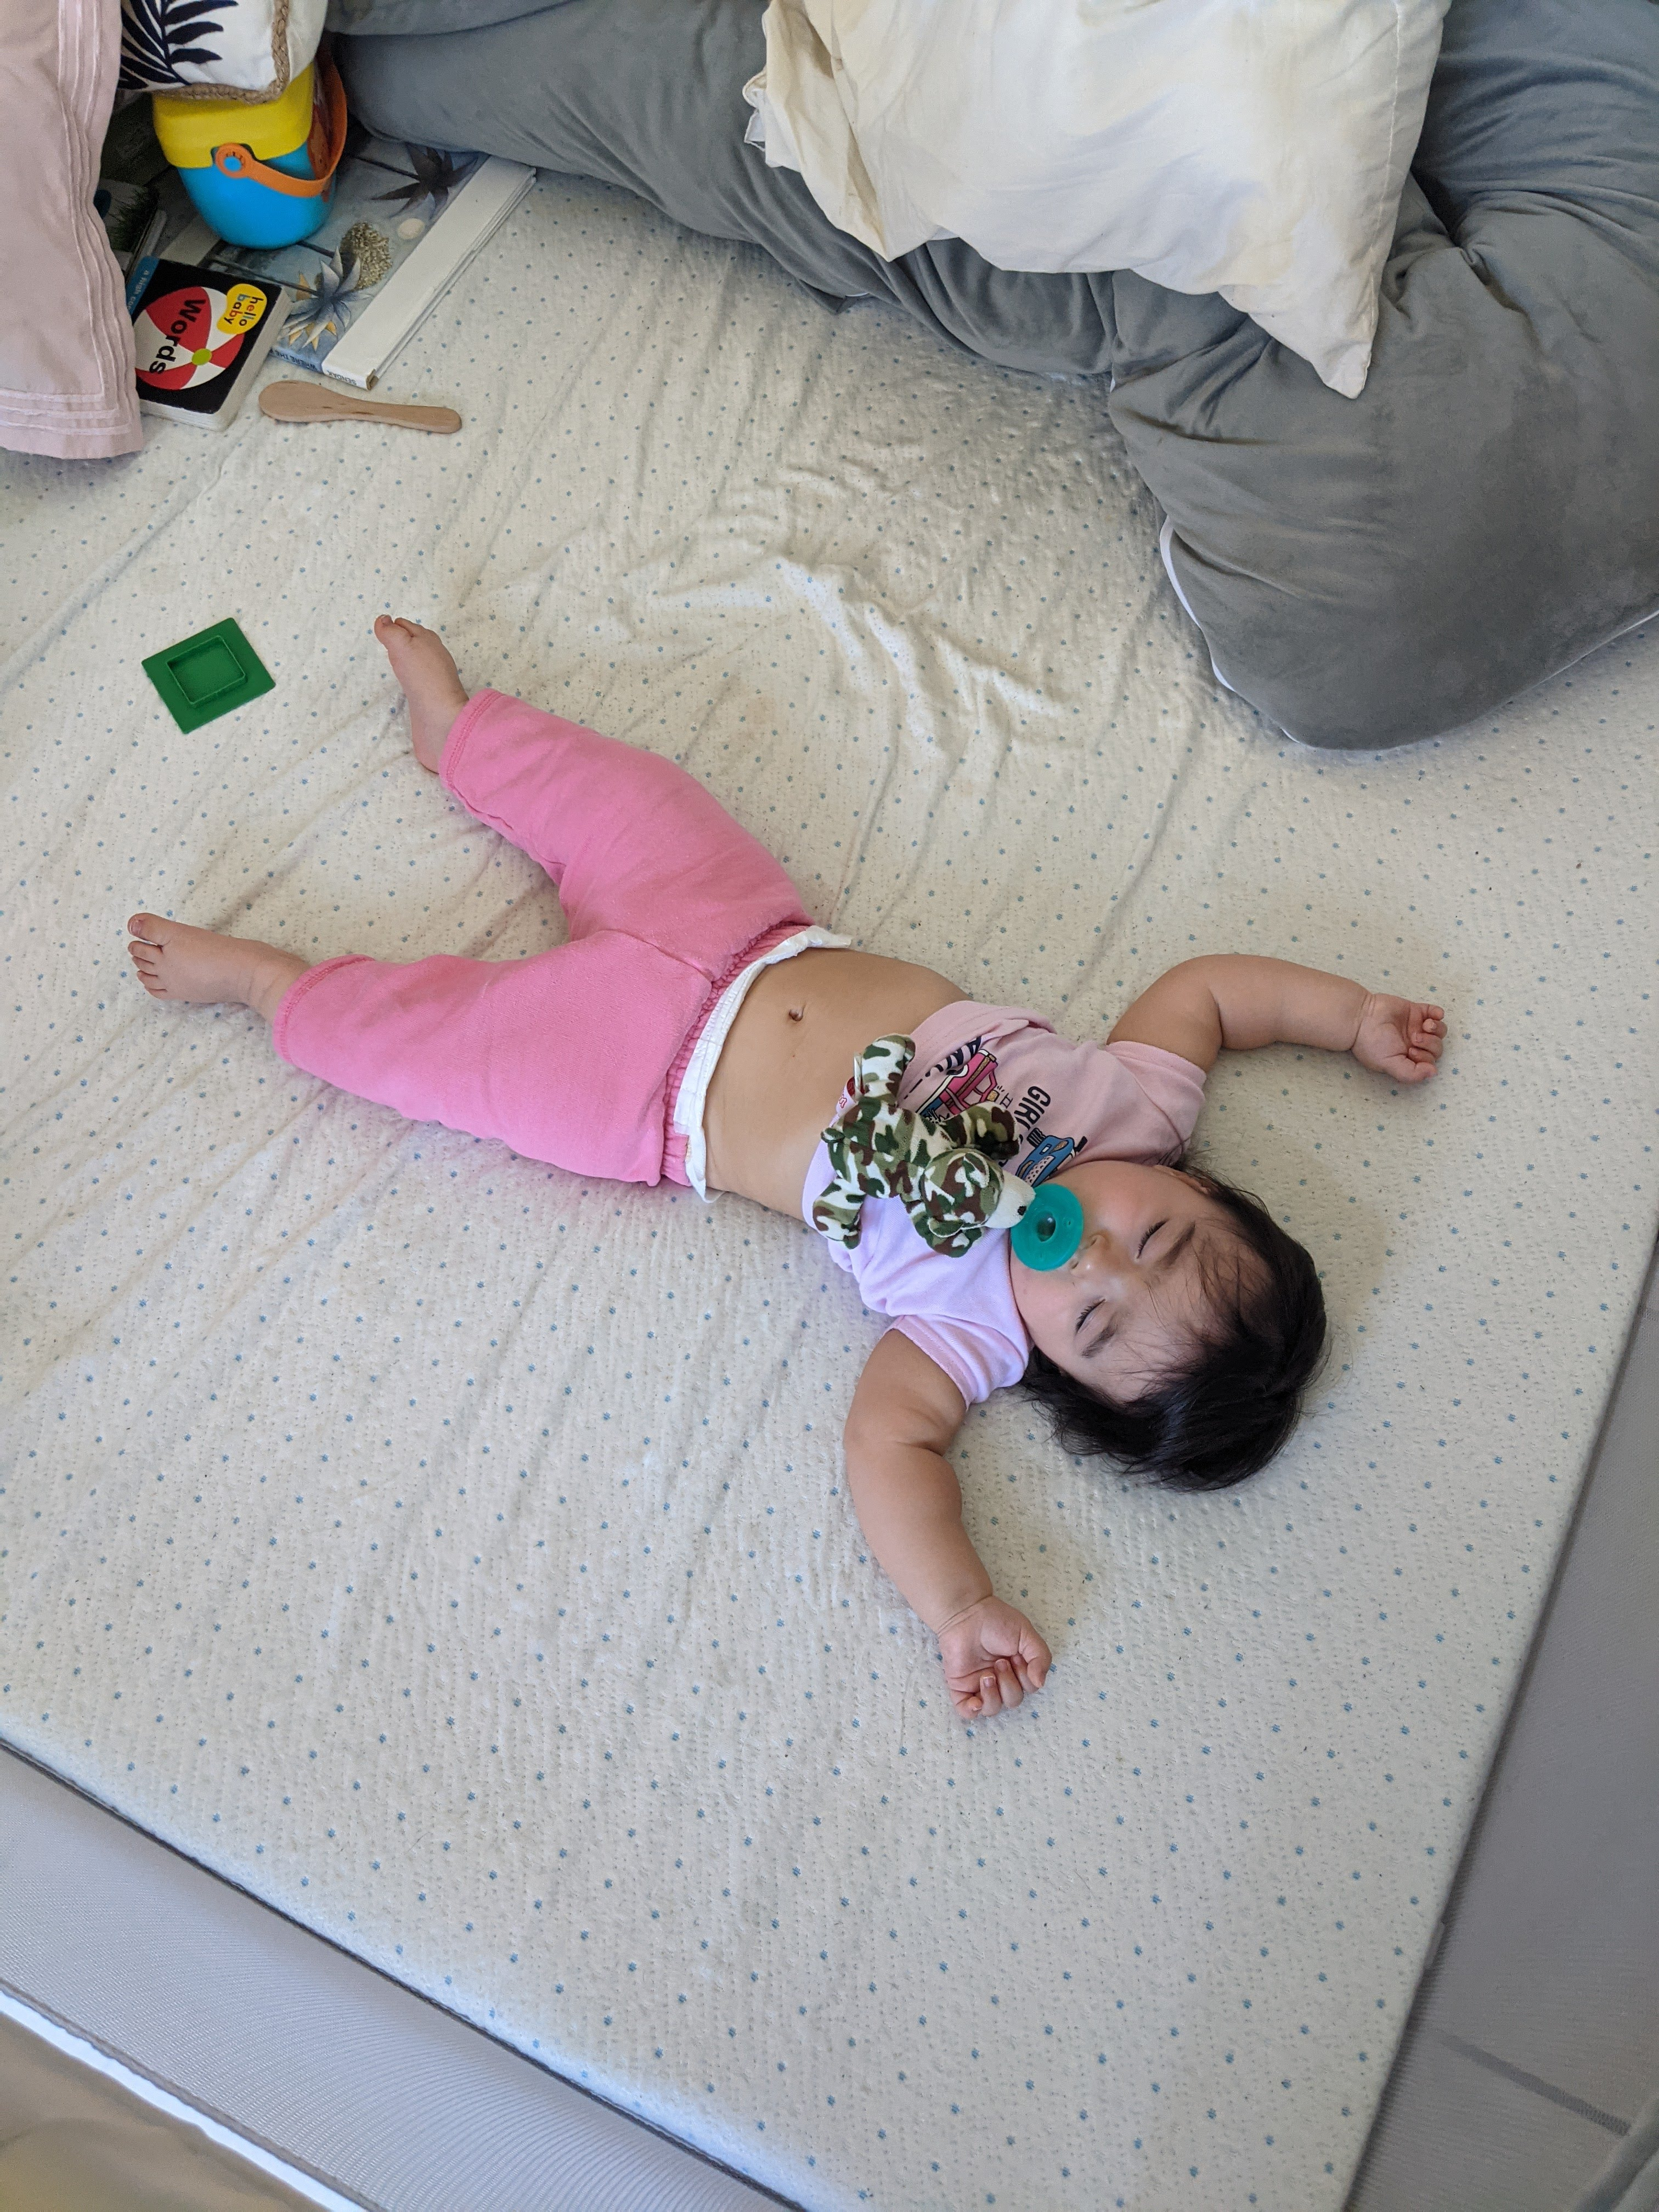
\includegraphics[width=0.5\textwidth]{sleep.jpg}
\end{figure}
\end{frame}

\begin{frame}{Whittier College}
\begin{figure}
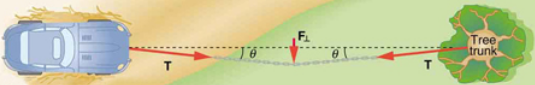
\includegraphics[width=0.5\textwidth]{tree.jpg}
\end{figure}
\end{frame}

\begin{frame}{Whittier College}
\begin{figure}
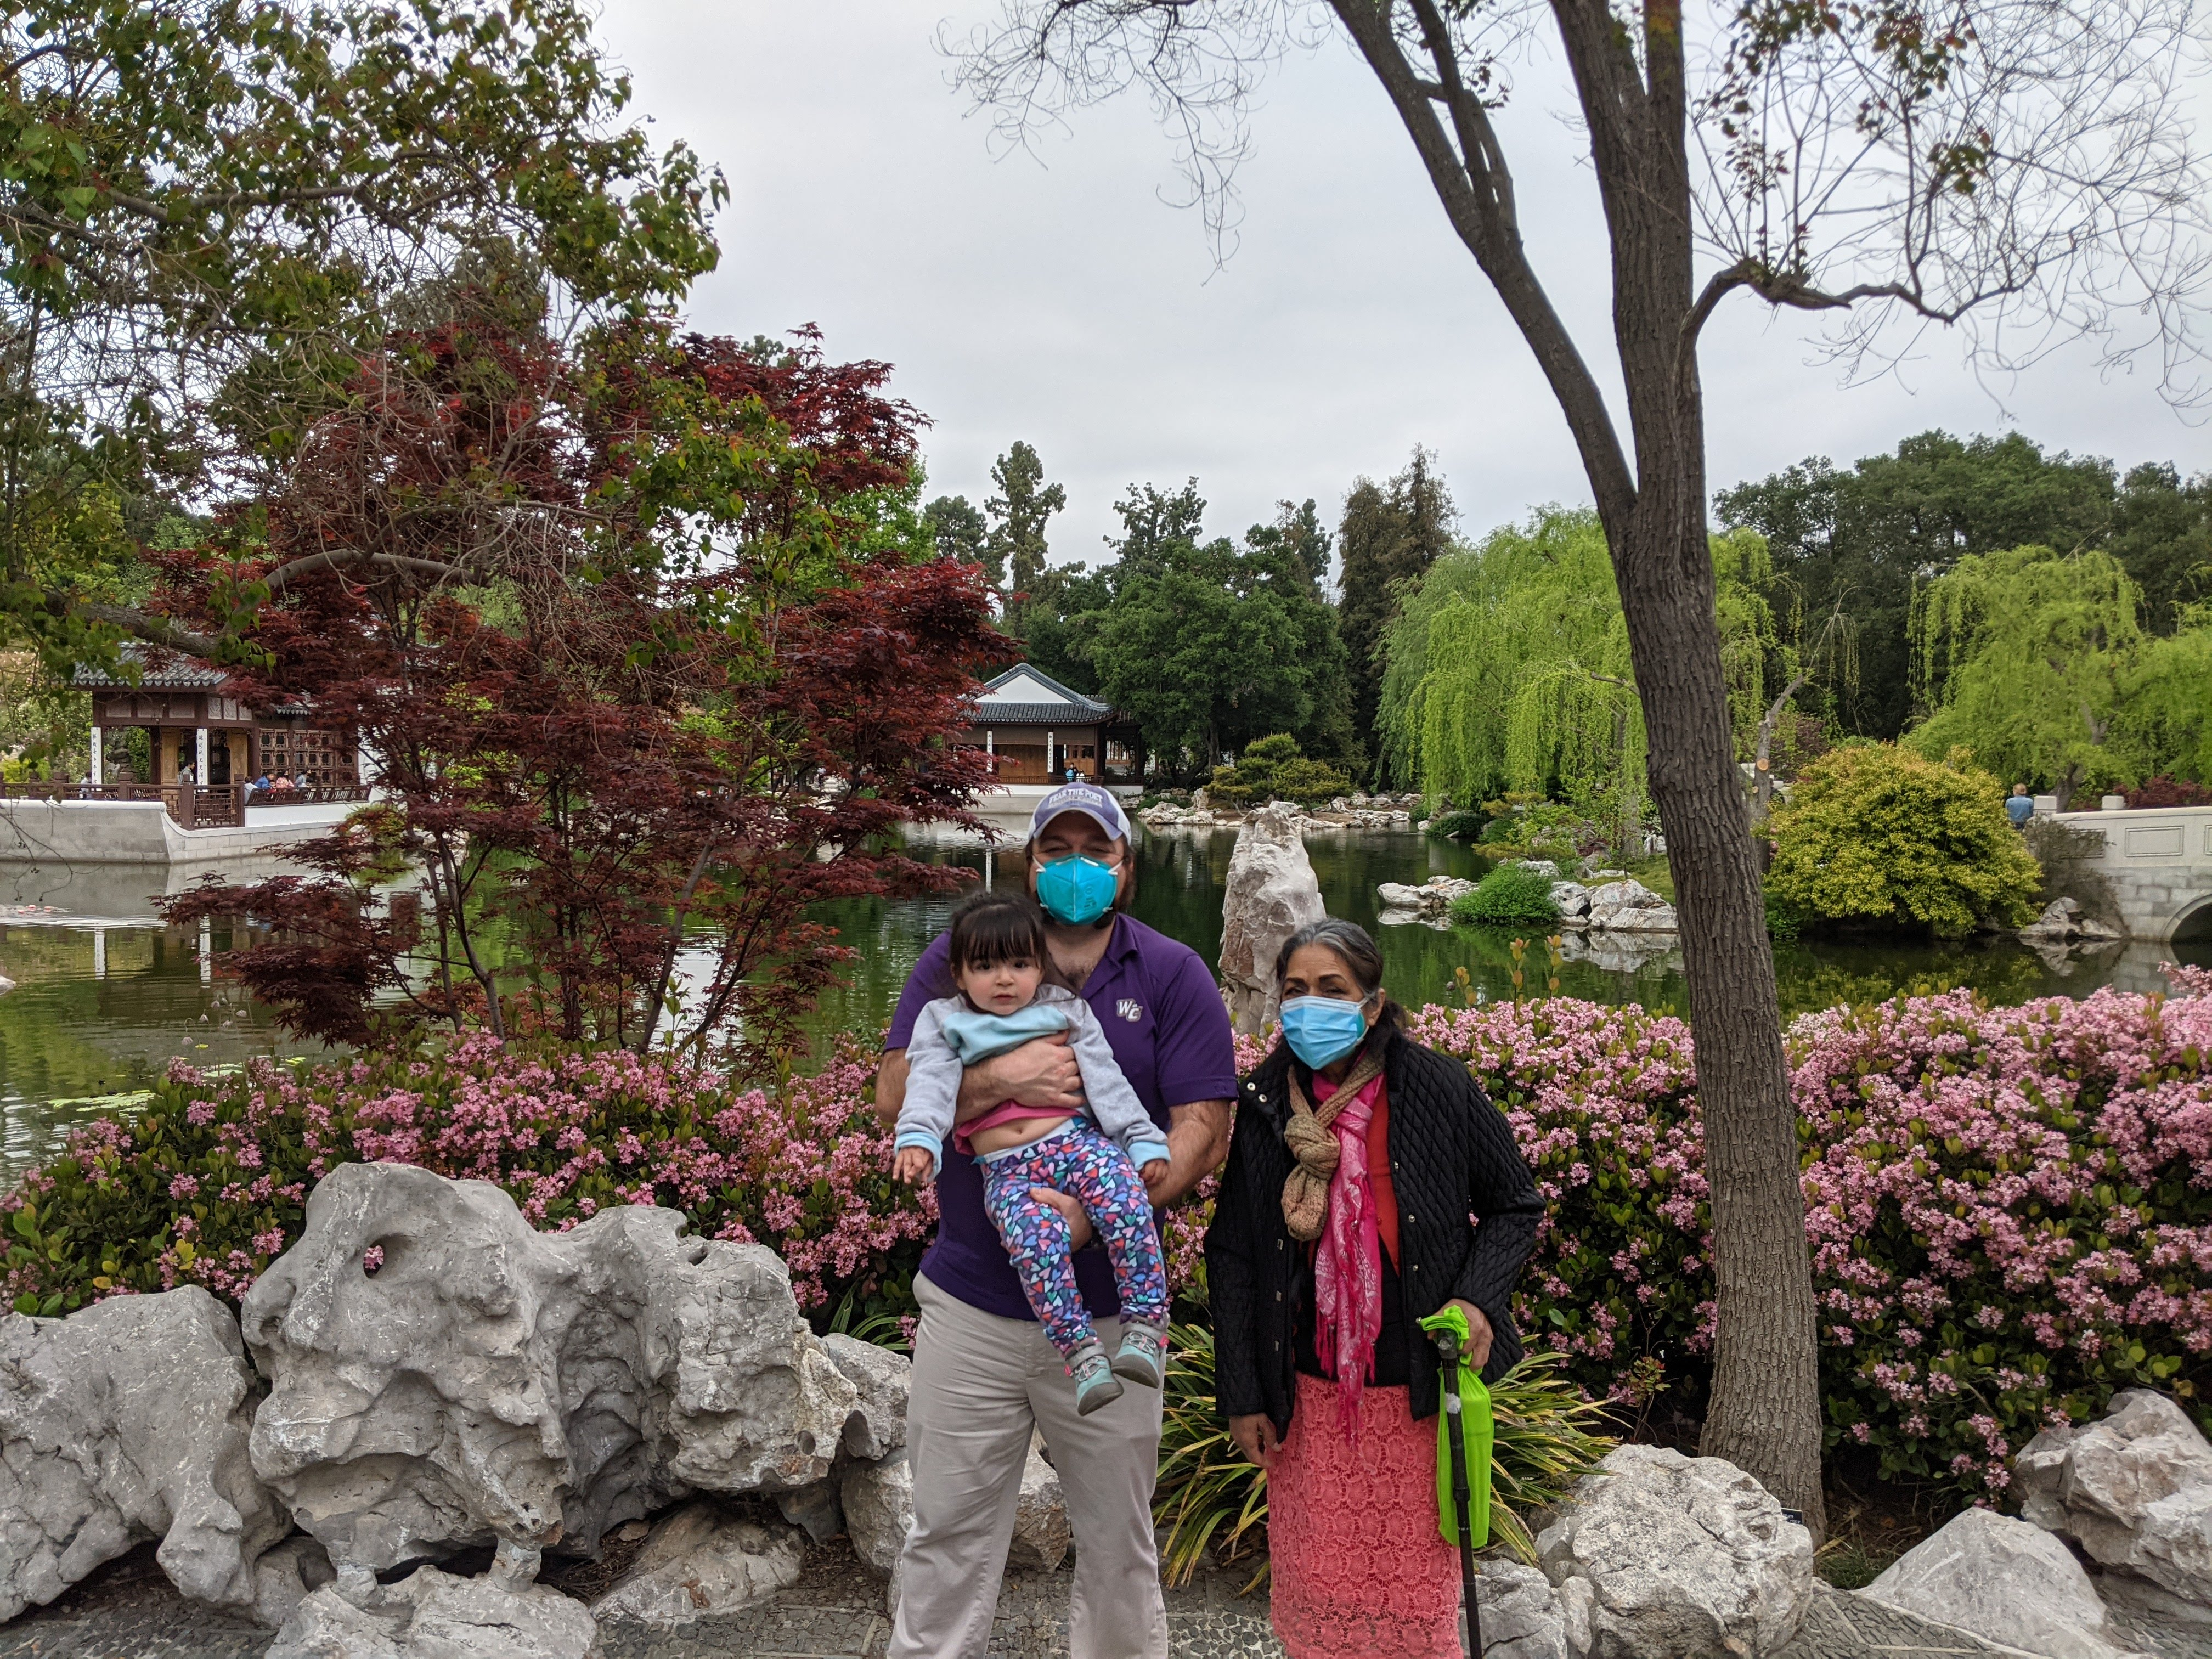
\includegraphics[width=0.85\textwidth]{photo1.jpg}
\end{figure}
\end{frame}

\begin{frame}{Whittier College}
\begin{figure}
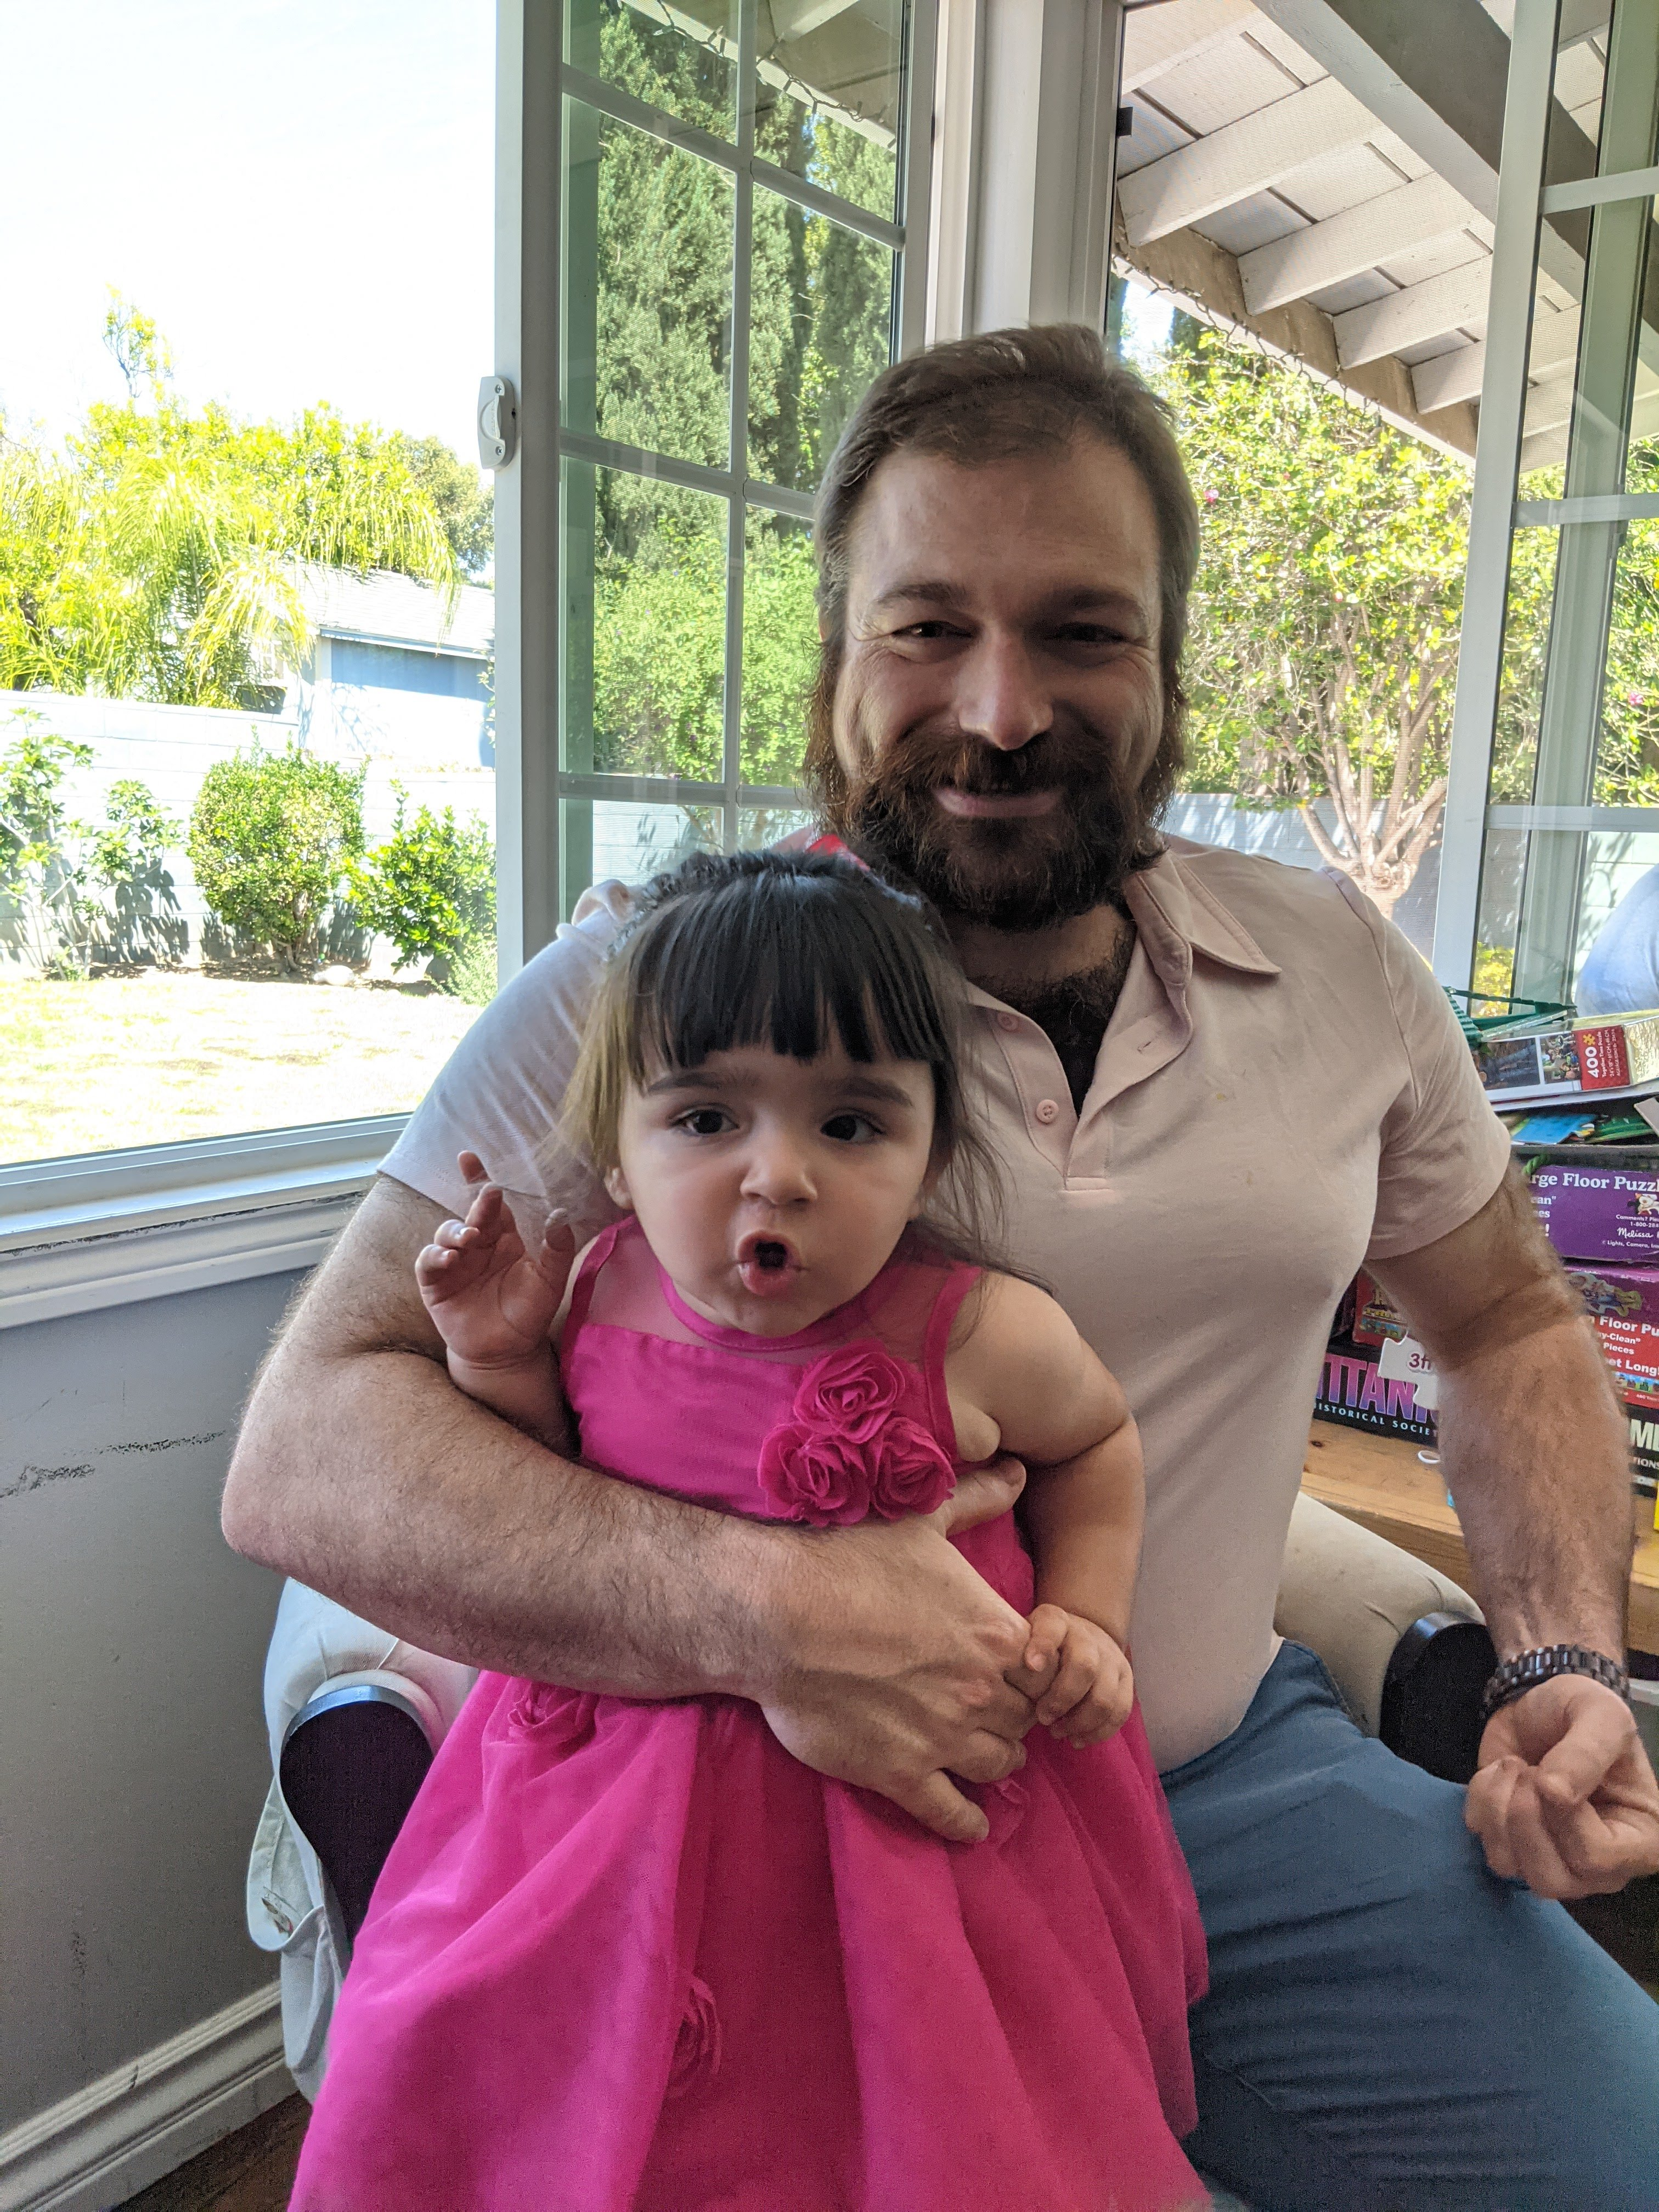
\includegraphics[width=0.5\textwidth]{photo2.jpg}
\end{figure}
\end{frame}


\section{Thank you.}

\end{document}
